%! Licence = CC BY-NC-SA 4.0

%! Author = gianfluetsch
%! Date = 22. Jan 2022
%! Project = icth_summary

\section{Fourieranalyse}

\subsubsection{A}
Konstruieren Sie ein System, das 5 harmonische Schwingungen addieren und sowohl im Zeit- als auch im Frequenzbereich darstellen kann. Bei jeder dieser Schwingungen sind Amplitude (-1 bis 1V), Frequenz (0 bis 200Hz) und Phase (0 bis 360 Grad) individuell via Handregler einstellbar.\\

Konstruieren sie nun das durch die Zerlegung unten dargestellte Signal. Was für eine Signalform entsteht? Beachten Sie, das Argument der SinusFunktion ist als Phasenwinkel angegeben.
Überführen sie die Sinusfunktion erst in eine Funktion der Zeit.\\
$S(x)=sin(x)-\frac{1}{2}sin(2x)+\frac{1}{3}sin(3x)-\frac{1}{4}sin(4x)$\\
$S(t)=sin(2\pi f_0t)-\frac{1}{2}sin(2\pi 2f_0t)+\frac{1}{3}sin(2\pi 3f_0t)-\frac{1}{4}sin(2\pi 4f_0t)$\\
Es entsteht ein Sägezahnsignal ($f_0=1kHz$).
\begin{center}
    \vspace{-8pt}
    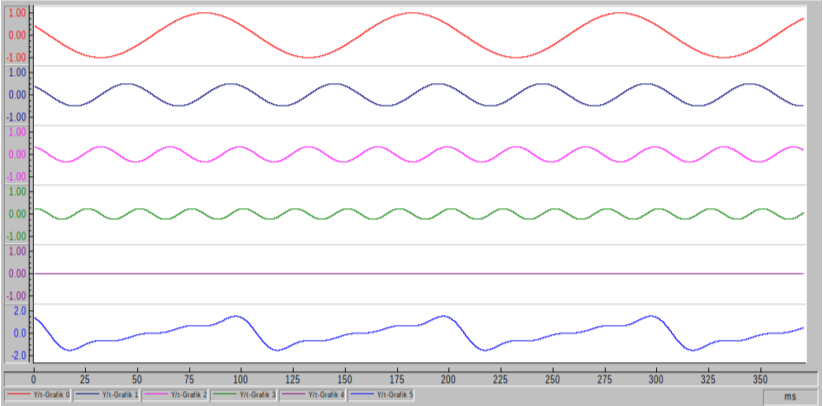
\includegraphics[width=.8\linewidth]{./14-fourieranalyse/w10}
    \vspace{-8pt}
\end{center}

Setzen sie die Reihe logisch fort. Was bedeutet das hinzufügen einer weitere Harmonischen (5. Harmonische)?\\
$S(t)=sin(2\pi f_0t)-\frac{1}{2}sin(2\pi 2f_0t)+\frac{1}{3}sin(2\pi 3f_0t)-\frac{1}{4}sin(2\pi 4f_0t)+\frac{1}{5}sin(2\pi 5f_0t)$\\
Das Signal nähert sich noch besser einem idealen Sägezahnsignal an!

Wie sieht das Spektrum des addierten Signales aus? Kann man das Spektrum unmittelbar aus der Fouriertransformierten ablesen?\\
Das Spektrum kann unmittelbar aus den Koeffizienten abgelesen werden:
\begin{center}
    \vspace{-8pt}
    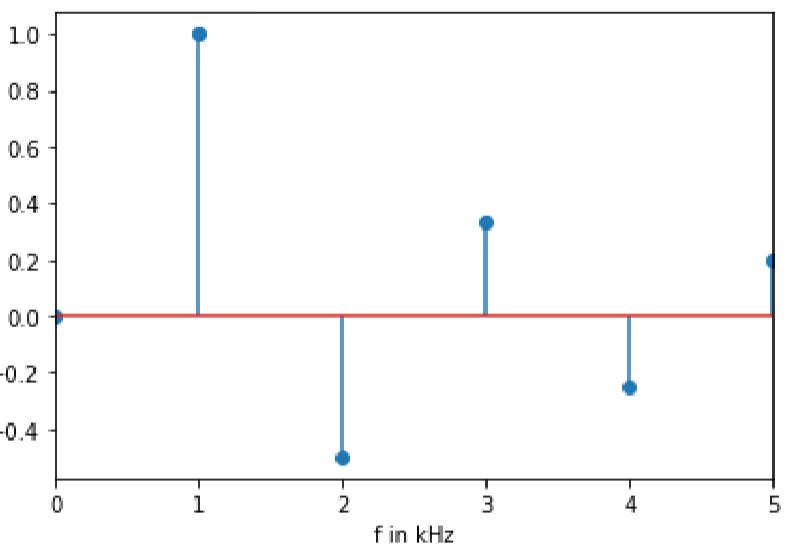
\includegraphics[width=.8\linewidth]{./14-fourieranalyse/w10_2}
    \vspace{-8pt}
\end{center}

\textbf{Untersuchen sie verschiedene Filtereinstellungen und Filtertypen TP, BP und HP. Welchen Einfluss haben diese und wie ver¨andert sich die Signalform des Ausgangssignales Sa(t)?}\\
\begin{itemize}
    \item TP: wie im Bild dargestellt, die Grundform ist noch erkennbar, da die Grundwelle noch enthalten ist.
    \item HP: hier ist im Ergebnis nicht mehr zur erkennen, was urspr¨unglich gesendet wurde, es sind nur die Summe der Oberwellen zu sehen.
    \item BP: je nach Einstellung ist nichts oder eine Anzahl überlagerter harmonischer Schwingungen zu sehen\\
\end{itemize}

\textbf{Was ändert sich, wenn sie die Frequenz des Generators verändern?}\\
Solange der Wert die Grenzfrequenz des TP nicht übersteigt, bleibt das Signal trotz stärker werdender Verzerrungen erkennbar. Wird bei steigender Generatorfrequenz ein stark beschneidender TP ausgewählt, bleibt nur noch
Rauschen.

\textbf{Was ändert sich, wenn sie die Amplitude ändern?}\\
Die Amplitude ändert sich linear mit.\\

\textbf{Können Sie das gleiche Problem mathematische mit Hilfe der Fourieranalyse (Tabelle) lösen (nur TP)?
Kontstruieren Sie den Verlauf des Ausgangssignals $S_a(t)$}\\
Gemäss Formelblatt ergibt sich für das Spektrum der Rechteckimpulsfolge:\\
$S_a(t)=\frac{A}{2}+\frac{2A}{\pi}(sin(\omega_0t)+\frac{1}{3}sin(3\omega_0t)+\frac{1}{5}sin(\omega_0t)+...)$\\
Mit A = 5. Der ideale Tiefpass schneidet Signale grösser 5f0 = 5kHz ab, damit ergibt sich für das Spektrum:\\
$S_a(t)=\frac{5}{2}+\frac{10}{\pi}sin(2\pi f_0t)+\frac{10}{3\pi}sin(32\pi f_0t)+\frac{10}{5\pi}(s\pi f_0t)$\\
\begin{center}
    \vspace{-8pt}
    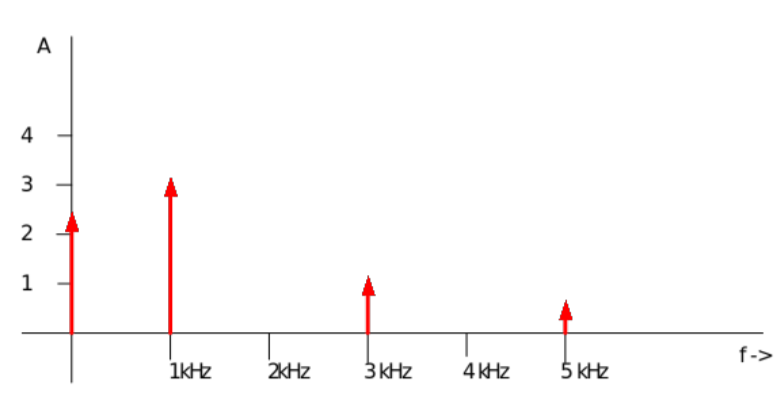
\includegraphics[width=.8\linewidth]{./14-fourieranalyse/w10_3}
    \vspace{-8pt}
\end{center}

Und damit das folgende Ausgangssignal:
\begin{center}
    \vspace{-8pt}
    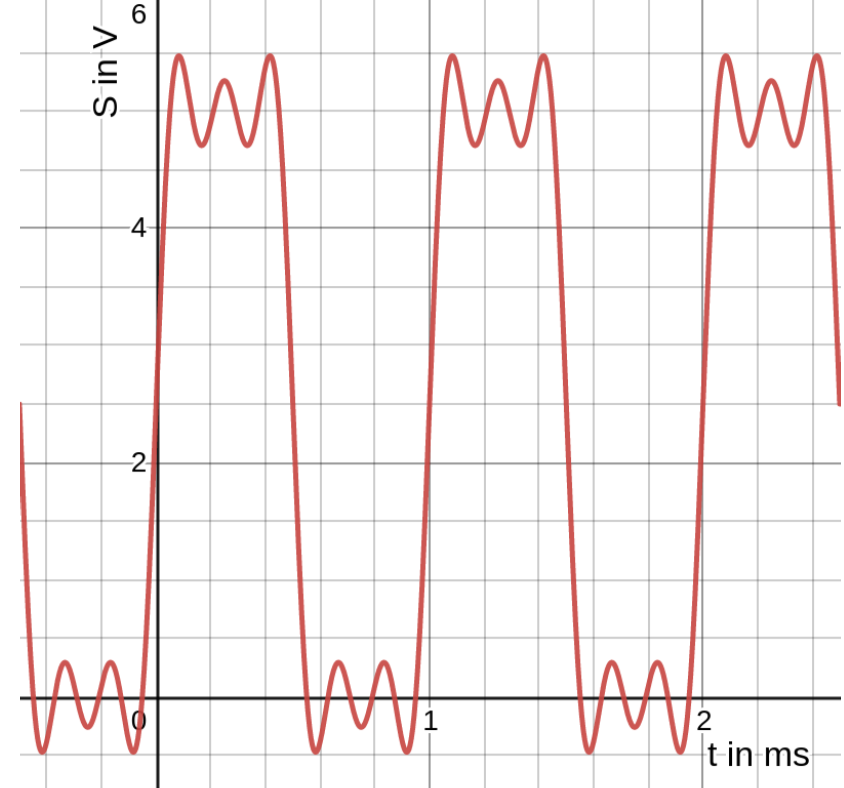
\includegraphics[width=.8\linewidth]{./14-fourieranalyse/w10_4}
    \vspace{-8pt}
\end{center}